
\documentclass[letterpaper,hide notes,xcolor={table,svgnames},pdftex,10pt]{beamer}
\def\showexamples{t}

\usecolortheme{crane}
\setbeamertemplate{navigation symbols}{}

\usetheme{MyPittsburgh}
\usepackage{hyperref}
\usepackage{graphicx,xspace}
\usepackage[normalem]{ulem}
\usepackage{multicol}
\usepackage{amsmath,amssymb,amsthm,graphicx,xspace}
\newcommand\SF[1]{$\bigstar$\footnote{SF: #1}}

\usepackage[sfdefault,lf]{carlito}
\usepackage[T1]{fontenc}
\usepackage[scaled]{beramono}
\usepackage{tikzpagenodes}
\newcommand{\Rplus}{\protect\hspace{-.1em}\protect\raisebox{.35ex}{\small{\small\textbf{+}}}}
\newcommand{\Cpp}{\mbox{C\Rplus\Rplus}\xspace}

\newcounter{tmpnumSlide}
\newcounter{tmpnumNote}

\newcommand\mnote[1]{%
	\addtocounter{tmpnumSlide}{1}
	\ifdefined\showcues {~\tiny\fbox{\arabic{tmpnumSlide}}}\fi
	\note{\setlength{\parskip}{1ex}\addtocounter{tmpnumNote}{1}\textbf{\Large \arabic{tmpnumNote}:} {#1\par}}}

\newcommand\mmnote[1]{\note{\setlength{\parskip}{1ex}#1\par}}


\newcommand\mquestion[2]{{~\color{red}\fbox{?}}\note{\setlength{\parskip}{1ex}\par{\Large \textbf{?}} #1} \note{\setlength{\parskip}{1ex}\par{\Large \textbf{A}} #2\par}\ifdefined \presentationonly \pause \fi}

\newcommand\blackboard[1]{%
	\ifdefined   \showblackboard
		{#1}
	\else {\begin{center} \fbox{\colorbox{blue!30}{%
						\begin{minipage}{.95\linewidth}%
							\hspace{\stretch{1}} Some space intentionally left blank; done at the blackboard.%
						\end{minipage}}}\end{center}}%
	\fi%
}

\usepackage{listings}
\lstset{%
	keywordstyle=\bfseries,
	aboveskip=15pt,
	belowskip=15pt,
	captionpos=b,
	identifierstyle=\ttfamily,
	frame=lines,
	numbers=left, basicstyle=\scriptsize, numberstyle=\tiny, stepnumber=0, numbersep=2pt}

\usepackage{siunitx}
\newcommand\sius[1]{\num[group-separator = {,}]{#1}\si{\micro\second}}
\newcommand\sims[1]{\num[group-separator = {,}]{#1}\si{\milli\second}}
\newcommand\sins[1]{\num[group-separator = {,}]{#1}\si{\nano\second}}
\sisetup{group-separator = {,}, group-digits = true}

%% -------------------- tikz --------------------
\usepackage{tikz}
\usetikzlibrary{positioning}
\usetikzlibrary{arrows,backgrounds,automata,decorations.shapes,decorations.pathmorphing,decorations.markings,decorations.text}

\tikzstyle{place}=[circle,draw=blue!50,fill=blue!20,thick, inner sep=0pt,minimum size=6mm]
\tikzstyle{transition}=[rectangle,draw=black!50,fill=black!20,thick, inner sep=0pt,minimum size=4mm]

\tikzstyle{block}=[rectangle,draw=black, thick, inner sep=5pt]
\tikzstyle{bullet}=[circle,draw=black, fill=black, thin, inner sep=2pt]

\tikzstyle{pre}=[<-,shorten <=1pt,>=stealth',semithick]
\tikzstyle{post}=[->,shorten >=1pt,>=stealth',semithick]
\tikzstyle{bi}=[<->,shorten >=1pt,shorten <=1pt, >=stealth',semithick]

\tikzstyle{mut}=[-,>=stealth',semithick]

\tikzstyle{treereset}=[dashed,->, shorten >=1pt,>=stealth',thin]

\usepackage{ifmtarg}
\usepackage{xifthen}
\makeatletter
% new counter to now which frame it is within the sequence
\newcounter{multiframecounter}
% initialize buffer for previously used frame title
\gdef\lastframetitle{\textit{undefined}}
% new environment for a multi-frame
\newenvironment{multiframe}[1][]{%
	\ifthenelse{\isempty{#1}}{%
		% if no frame title was set via optional parameter,
		% only increase sequence counter by 1
		\addtocounter{multiframecounter}{1}%
	}{%
		% new frame title has been provided, thus
		% reset sequence counter to 1 and buffer frame title for later use
		\setcounter{multiframecounter}{1}%
		\gdef\lastframetitle{#1}%
	}%
	% start conventional frame environment and
	% automatically set frame title followed by sequence counter
	\begin{frame}%
		\frametitle{\lastframetitle~{\normalfont(\arabic{multiframecounter})}}%
		}{%
	\end{frame}%
}
\makeatother

\makeatletter
\newdimen\tu@tmpa%
\newdimen\ydiffl%
\newdimen\xdiffl%
\newcommand\ydiff[2]{%
	\coordinate (tmpnamea) at (#1);%
	\coordinate (tmpnameb) at (#2);%
	\pgfextracty{\tu@tmpa}{\pgfpointanchor{tmpnamea}{center}}%
	\pgfextracty{\ydiffl}{\pgfpointanchor{tmpnameb}{center}}%
	\advance\ydiffl by -\tu@tmpa%
}
\newcommand\xdiff[2]{%
	\coordinate (tmpnamea) at (#1);%
	\coordinate (tmpnameb) at (#2);%
	\pgfextractx{\tu@tmpa}{\pgfpointanchor{tmpnamea}{center}}%
	\pgfextractx{\xdiffl}{\pgfpointanchor{tmpnameb}{center}}%
	\advance\xdiffl by -\tu@tmpa%
}
\makeatother
\newcommand{\copyrightbox}[3][r]{%
	\begin{tikzpicture}%
		\node[inner sep=0pt,minimum size=2em](ciimage){#2};
		\usefont{OT1}{phv}{n}{n}\fontsize{4}{4}\selectfont
		\ydiff{ciimage.south}{ciimage.north}
		\xdiff{ciimage.west}{ciimage.east}
		\ifthenelse{\equal{#1}{r}}{%
			\node[inner sep=0pt,right=1ex of ciimage.south east,anchor=north west,rotate=90]%
			{\raggedleft\color{black!50}\parbox{\the\ydiffl}{\raggedright{}#3}};%
		}{%
			\ifthenelse{\equal{#1}{l}}{%
				\node[inner sep=0pt,right=1ex of ciimage.south west,anchor=south west,rotate=90]%
				{\raggedleft\color{black!50}\parbox{\the\ydiffl}{\raggedright{}#3}};%
			}{%
				\node[inner sep=0pt,below=1ex of ciimage.south west,anchor=north west]%
				{\raggedleft\color{black!50}\parbox{\the\xdiffl}{\raggedright{}#3}};%
			}
		}
	\end{tikzpicture}
}


%% --------------------

%\usepackage[excludeor]{everyhook}
%\PushPreHook{par}{\setbox0=\lastbox\llap{MUH}}\box0}

%\vspace*{\stretch{1}

%\setbox0=\lastbox \llap{\textbullet\enskip}\box0}

\setlength{\parskip}{\fill}

\newcommand\noskips{\setlength{\parskip}{1ex}}
\newcommand\doskips{\setlength{\parskip}{\fill}}

\newcommand\xx{\par\vspace*{\stretch{1}}\par}
\newcommand\xxs{\par\vspace*{2ex}\par}
\newcommand\tuple[1]{\langle #1 \rangle}
\newcommand\code[1]{{\sf \footnotesize #1}}
\newcommand\ex[1]{\uline{Example:} \ifdefined \presentationonly \pause \fi
	\ifdefined\showexamples#1\xspace\else{\uline{\hspace*{2cm}}}\fi}

\newcommand\ceil[1]{\lceil #1 \rceil}


\AtBeginSection[]
{
	\begin{frame}
		\frametitle{Outline}
		\tableofcontents[currentsection]
	\end{frame}
}



\pgfdeclarelayer{edgelayer}
\pgfdeclarelayer{nodelayer}
\pgfsetlayers{edgelayer,nodelayer,main}

\tikzstyle{none}=[inner sep=0pt]
\tikzstyle{rn}=[circle,fill=Red,draw=Black,line width=0.8 pt]
\tikzstyle{gn}=[circle,fill=Lime,draw=Black,line width=0.8 pt]
\tikzstyle{yn}=[circle,fill=Yellow,draw=Black,line width=0.8 pt]
\tikzstyle{empty}=[circle,fill=White,draw=Black]
\tikzstyle{bw} = [rectangle, draw, fill=blue!20,
text width=4em, text centered, rounded corners, minimum height=2em]

\newcommand{\CcNote}[1]{% longname
	This work is licensed under the \textit{Creative Commons #1 3.0 License}.%
}
\newcommand{\CcImageBy}[1]{%
	\includegraphics[scale=#1]{creative_commons/cc_by_30.pdf}%
}
\newcommand{\CcImageSa}[1]{%
	\includegraphics[scale=#1]{creative_commons/cc_sa_30.pdf}%
}
\newcommand{\CcImageNc}[1]{%
	\includegraphics[scale=#1]{creative_commons/cc_nc_30.pdf}%
}
\newcommand{\CcGroupBySa}[2]{% zoom, gap
	\CcImageBy{#1}\hspace*{#2}\CcImageNc{#1}\hspace*{#2}\CcImageSa{#1}%
}
\newcommand{\CcLongnameByNcSa}{Attribution-NonCommercial-ShareAlike}

\newenvironment{changemargin}[1]{% 
	\begin{list}{}{% 
		\setlength{\topsep}{0pt}% 
		\setlength{\leftmargin}{#1}% 
		\setlength{\rightmargin}{1em}
		\setlength{\listparindent}{\parindent}% 
		\setlength{\itemindent}{\parindent}% 
		      \setlength{\parsep}{\parskip}% 
		      }% 
		\item[]}{\end{list}}




\title{Lecture 26 --- Virtualization and Containers }

\author{Jeff Zarnett \\ \small \texttt{jzarnett@uwaterloo.ca}}
\institute{Department of Electrical and Computer Engineering \\
  University of Waterloo}
\date{\today}


\begin{document}

\begin{frame}
  \titlepage

 \end{frame}



\begin{frame}
\frametitle{Virtualization and Virtual Machines}

The word virtualization itself can refer to many different aspects of computing.

\begin{center}
	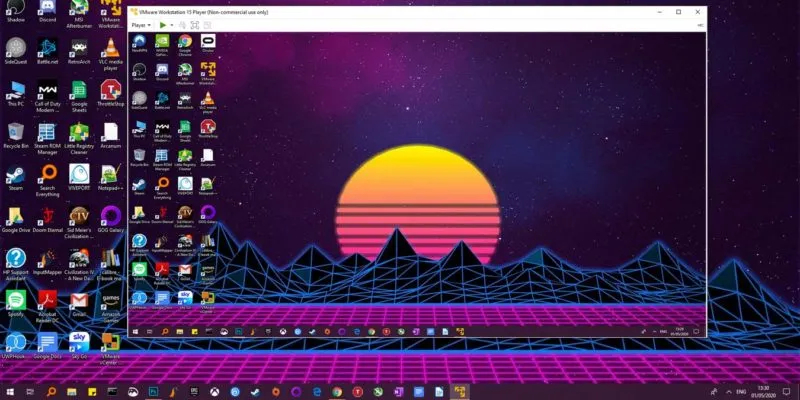
\includegraphics[width=\textwidth]{images/virtualmachine.jpg}
\end{center}

The part that we really want to talk about is ``virtual machines''. 

 \end{frame}



\begin{frame}
\frametitle{Virtualization and Virtual Machines}

The goal is to abstract the hardware of a single computer into several different execution environments. 

We might have different operating systems running, or multiple copies of the same operating system, depending on what is desired. 

\end{frame}

\begin{frame}
\frametitle{Enter the Matrix}

From the perspective of the operating system, however, it does not usually know that it is executing on an abstraction of the hardware. 


\begin{center}
	
\includegraphics[width=0.7\textwidth]{images/redbluepill.jpg}
\end{center}

``How would you know the difference between the dream world and the real world?''


\end{frame}

\begin{frame}
\frametitle{The Host and the VMM}


At the lowest level, there is the \alert{host}, the underlying hardware system. 

Above that is the \alert{virtual machine manager} (VMM) or \alert{hypervisor}.

The VMM creates an interface that looks like the host. 

The \alert{guests} interact with their own virtual copy of the host.

\end{frame}

\begin{frame}
\frametitle{Virtual and Non-Virtual Machine}

\begin{center}
	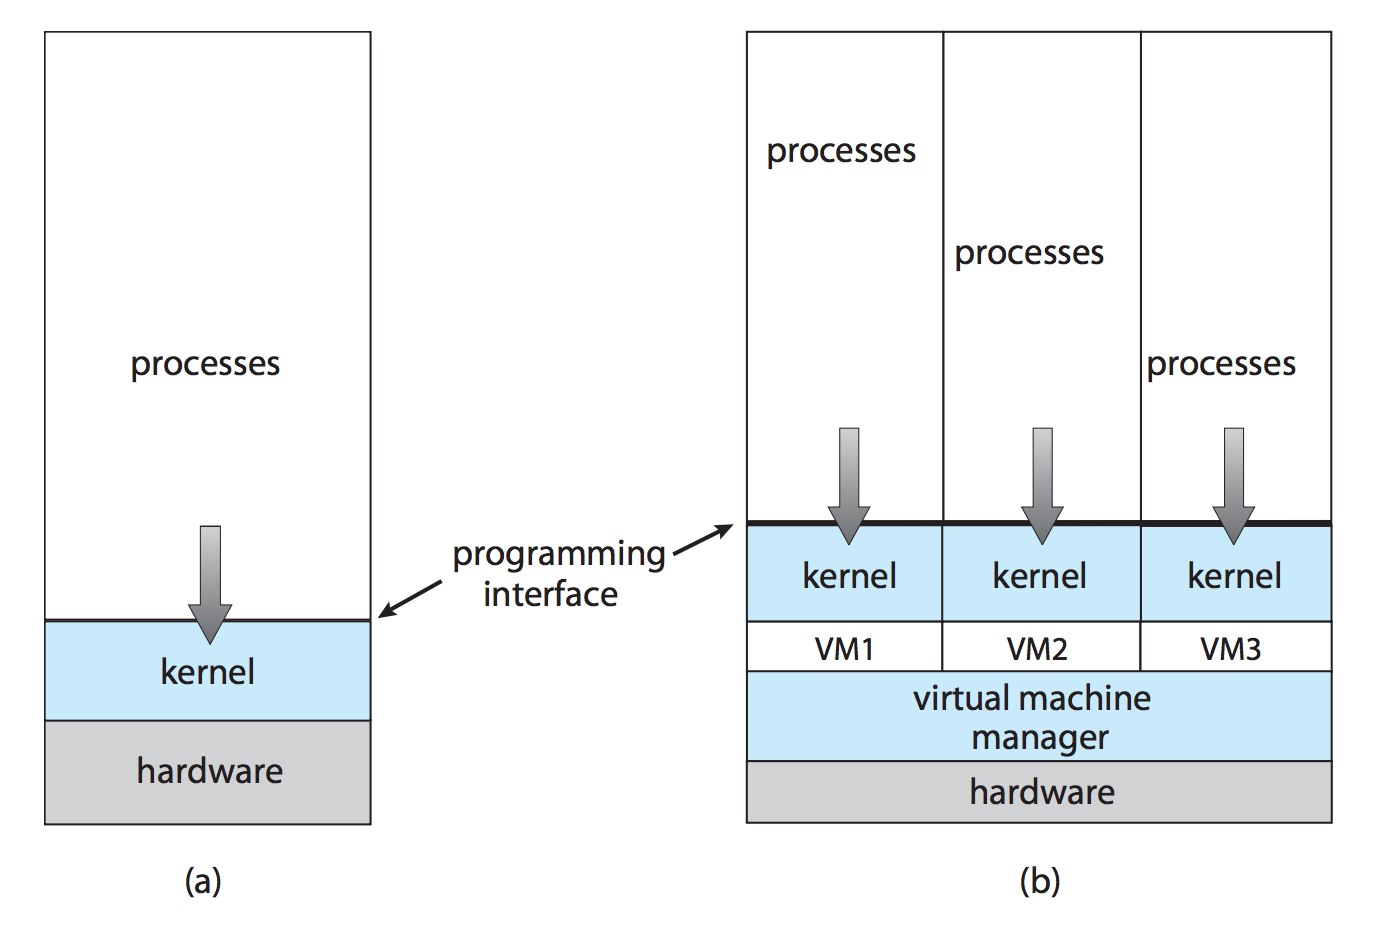
\includegraphics[width=0.8\textwidth]{images/non-virtual-machine.png}
\end{center}

\end{frame}

\begin{frame}
\frametitle{Emulation}

This is by no means the same thing as \alert{emulation}. 

When we have virtualization both Windows and Linux can be running on the same x86\_64 architecture as guests. 

In the case of the Android emulator running in an x86\_64 machine: 

The code of the emulator is running on the x86\_64 environment to simulate an Android hardware device that would have a completely different CPU. 

\end{frame}

\begin{frame}
\frametitle{Emulation}

Thus, an Android app (which would not otherwise run on an Intel/AMD machine) runs in a simulation of a mobile environment. 

The emulation operation is incredibly slow, unfortunately, as anyone who has tried to use the Android emulator has found out. 

If you are trying to play a classic game that ran under MS-DOS, emulating a 486 computer does not take much by way of resources.



\end{frame}

\begin{frame}
\frametitle{Requires Windows XP}

Use an OS other than Windows? 

You are likely to have had the situation where one or more programs that are needed for some purpose (work, school...) function only under Windows. 

\end{frame}

\begin{frame}
\frametitle{Requires Windows XP}

And as the versions of Windows have proliferated and evolved, older programs have sometimes stopped working.

\begin{center}
	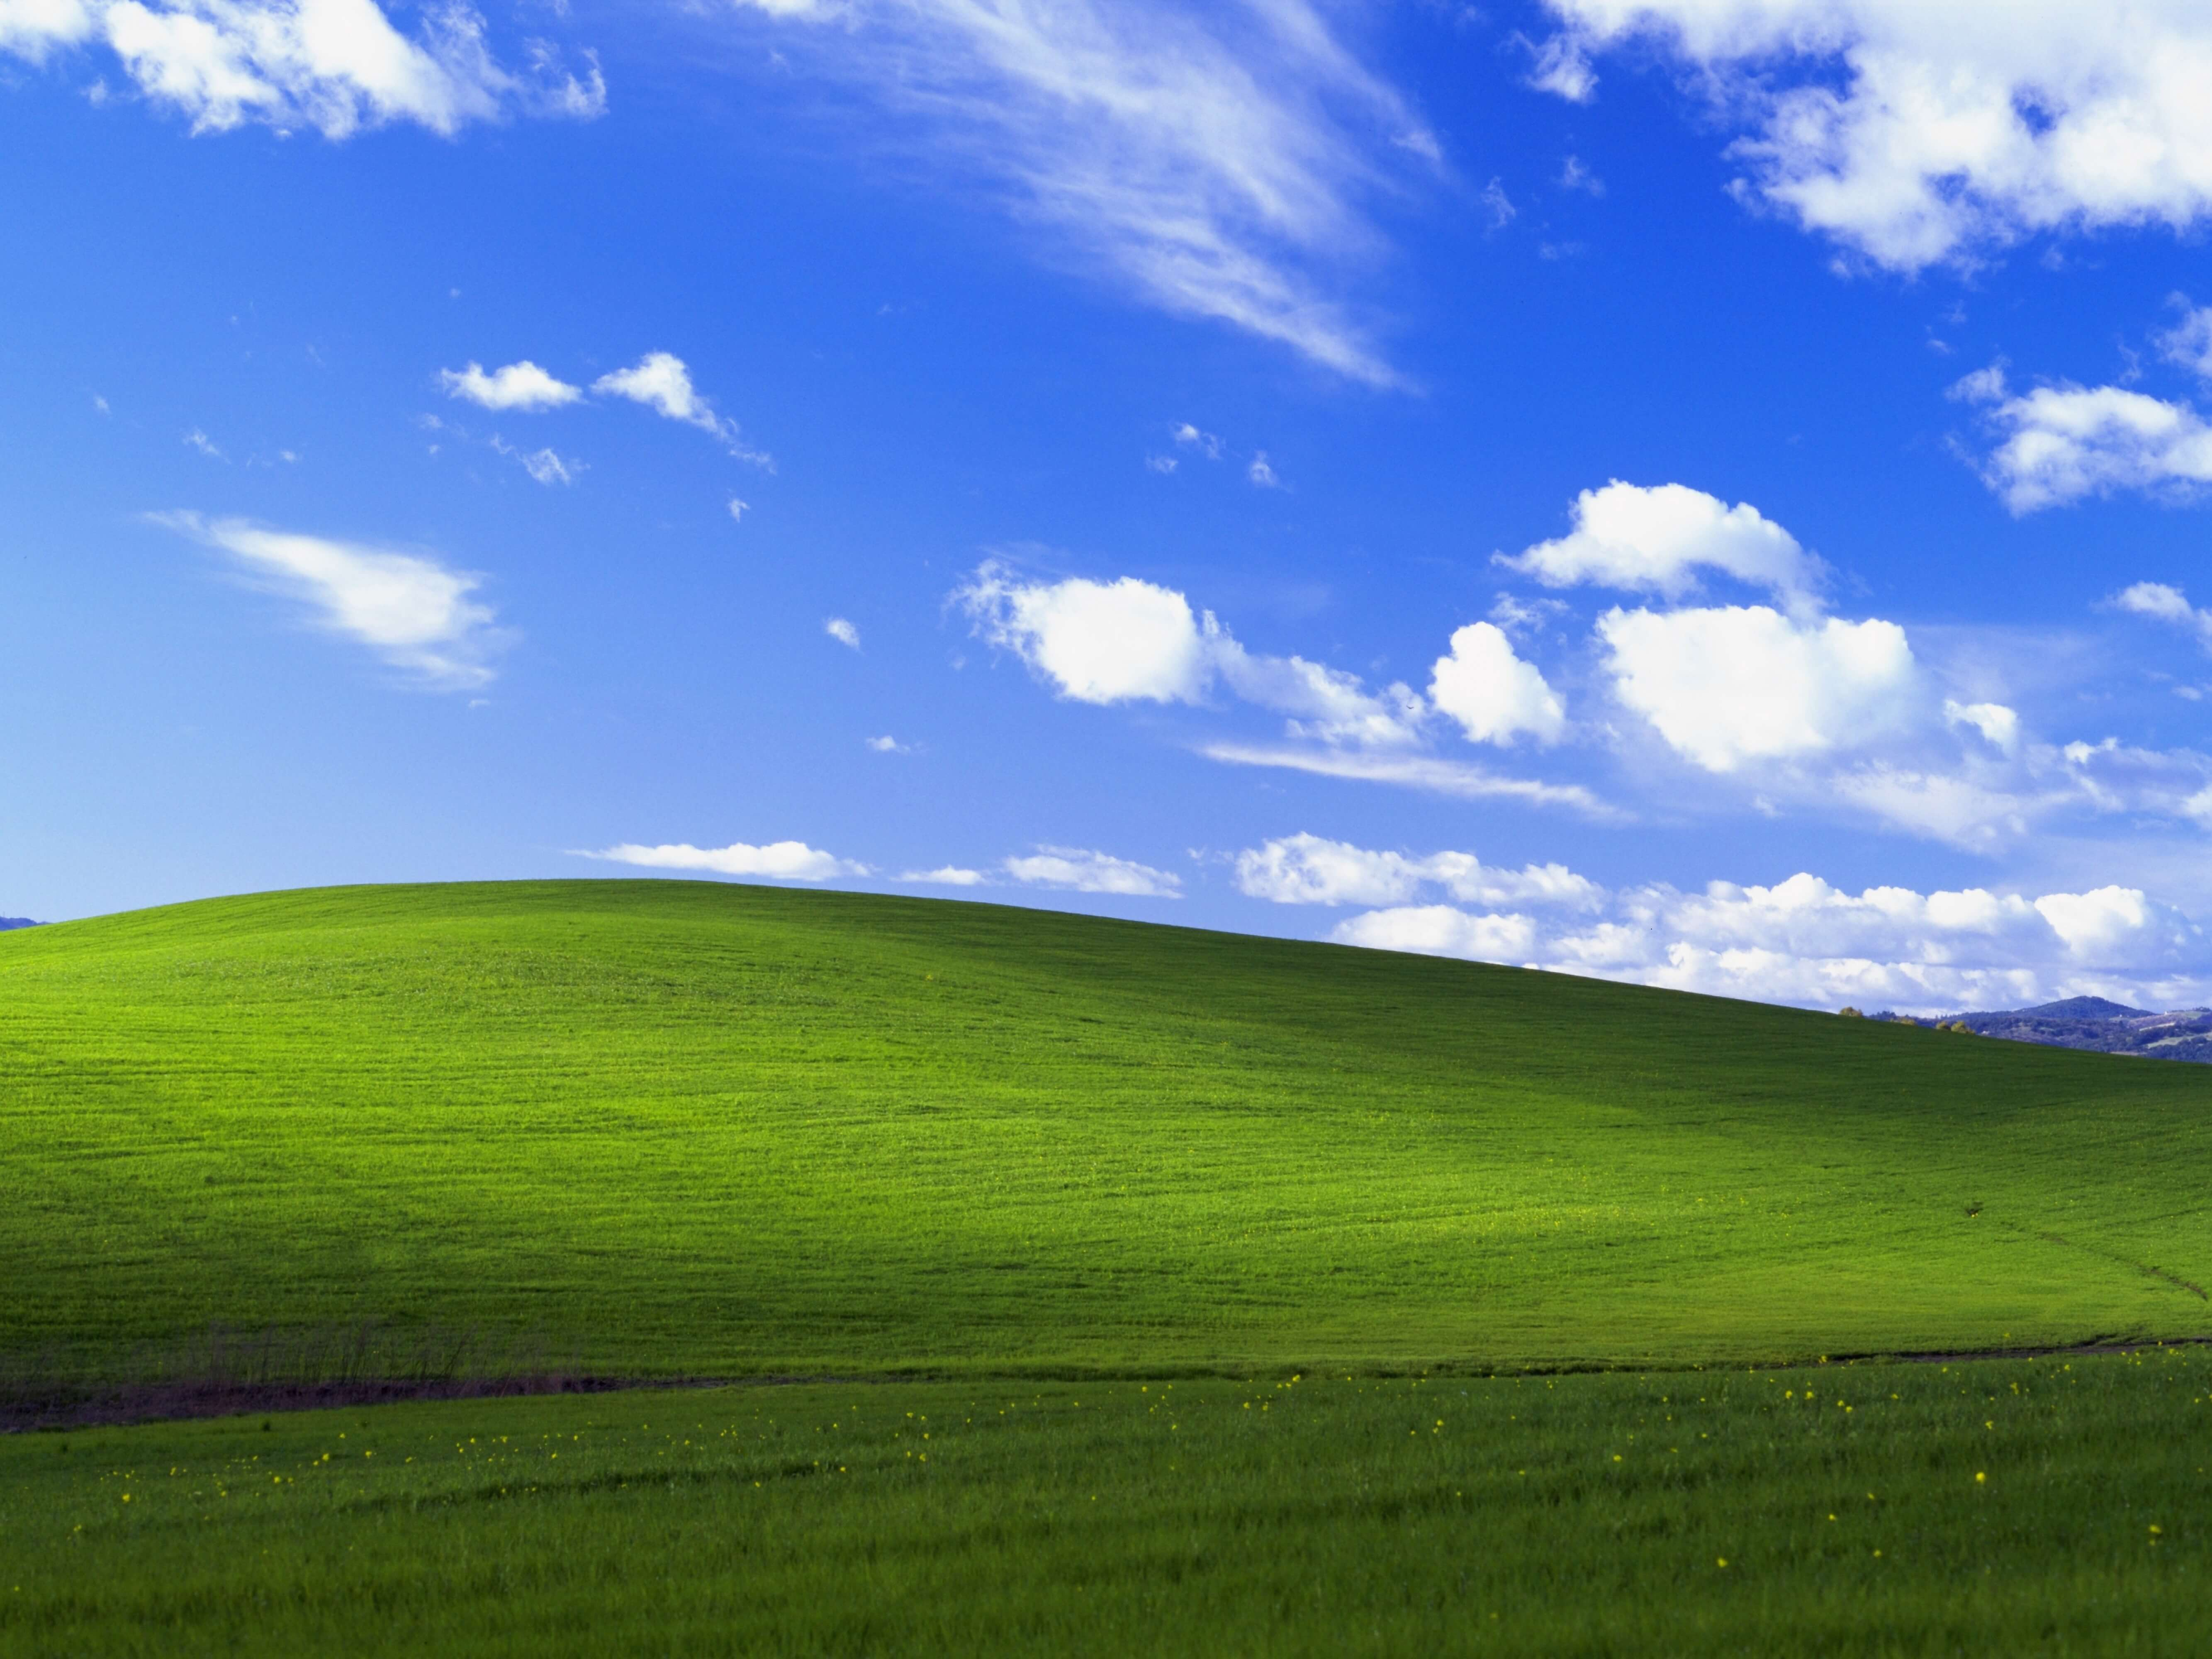
\includegraphics[width=0.5\textwidth]{images/winxp.jpg}
\end{center}

So this necessitates a past version (Windows XP will never, ever die...).

\end{frame}

\begin{frame}
\frametitle{Pause and Play}

Another neat thing is the ability to suspend (pause) execution. 

This is like pausing a process: the current state is taken and saved, and can be restored at a later time. 

Also like a process, it can be moved around to another system and resume after that move has taken place, or cloned to get an identical copy somewhere else.


\end{frame}

\begin{frame}
\frametitle{Protection}

A third reason for virtualization is protection. 

The guests are isolated from the host and vice versa. 

If a virus infects one of the guests, the other guests are not affected. 

\end{frame}

\begin{frame}
\frametitle{Protection}

And with a virtual machine, it will be that much easier to delete and reinstall the guest or roll it back to an earlier state. 

This would be exactly the state that we have stored when suspending it...


\end{frame}

\begin{frame}
\frametitle{Consolidation}


Many servers running that could be sharing the same physical hardware. 

Instead of having a lot of lightly used physical systems, convert them to virtual and put them all in the same physical machine. 


\end{frame}

\begin{frame}
\frametitle{Behind the Scenes: VCPU}

One of the key building blocks of virtualization is the \alert{virtual CPU} (VCPU). 

It does not execute code; it is the state of the CPU according to the guest. 

The VMM is responsible for maintaining the state of the VCPU. 

Much like the process control block, the VCPU is a data structure that is used to store the state when the guest is not running.

The state is restored from the VCPU when the guest is scheduled to run.

\end{frame}

\begin{frame}
\frametitle{User and Kernel Mode}

Application processes run in user mode and the kernel runs in kernel mode, having access to privileged instructions. 

The guest operating system runs in user mode, but it will want to do some things that require kernel mode.

So we will need to have virtual user mode and virtual kernel mode.

\end{frame}

\begin{frame}
\frametitle{Trap-and-Emulate}

If the guest attempts a privileged instruction, it will generate a trap (error) because it is in user mode. 

The VMM should then pick this up and executes, emulating (or simulating, if you prefer) the requested operation.

\end{frame}

\begin{frame}
\frametitle{Trap-and-Emulate}

\begin{center}
	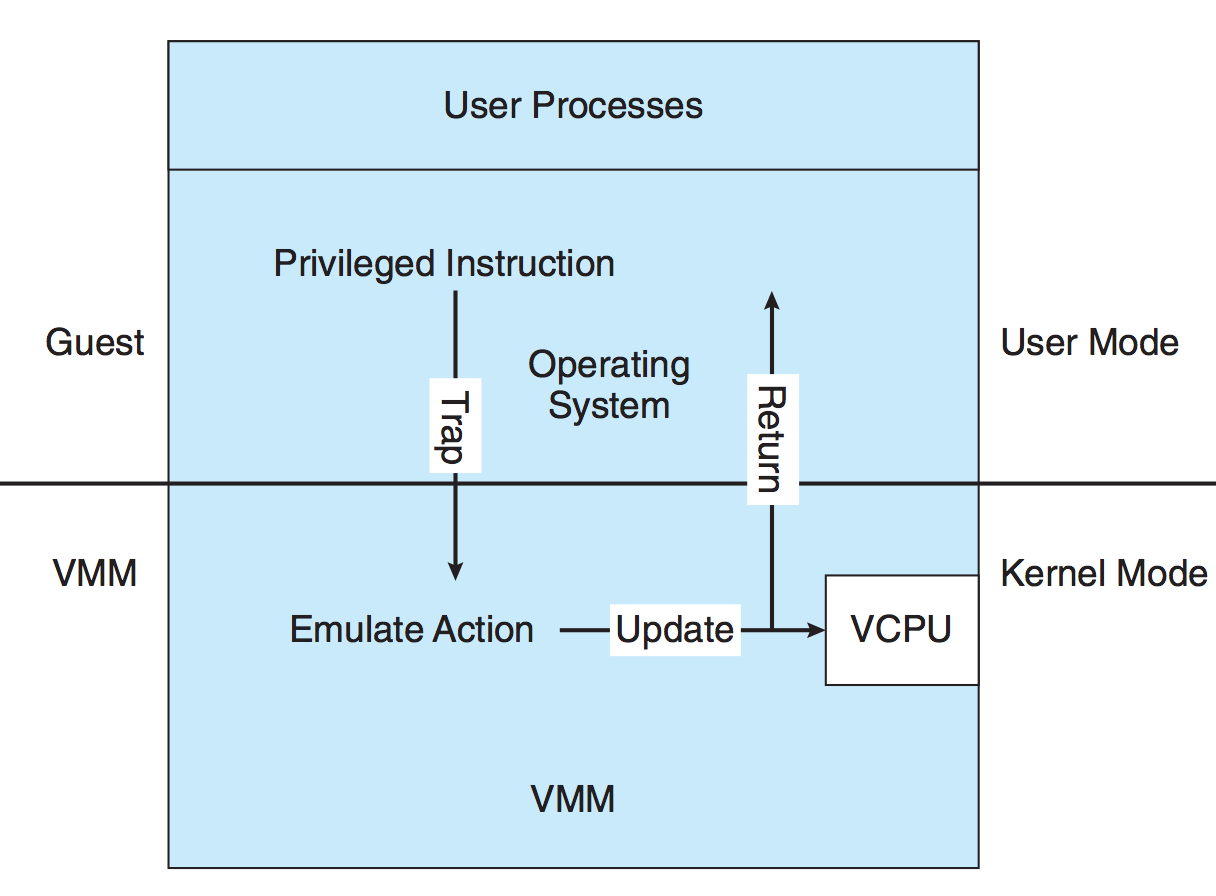
\includegraphics[width=0.75\textwidth]{images/trap-and-emulate.png}
\end{center}

\end{frame}

\begin{frame}
\frametitle{Trap-and-Emulate Speed}

Non-privileged instructions just execute natively on the hardware; they are as fast as they would be if they were being executed outside a virtual machine. 

Unfortunately, with trap-and-emulate, privileged instructions have this extra overhead, causing the guest to run more slowly than it otherwise would. 

\end{frame}

\begin{frame}
\frametitle{Trap-and-Emulate Speed}

Hardware designers have come to the rescue again: some CPUs have more than just the two simple modes (user/kernel).

They keep track in hardware of virtual user and virtual kernel mode. 

That relieves the VMM from the responsibility of keeping track of it.


\end{frame}

\begin{frame}
\frametitle{There's a Catch...}

Sadly, some CPUs do not have clear definitions of privileged vs. non-privileged instructions, including the intel x86 architecture. 

There were a lot of decisions that make no sense if we look at them with what we know today, but they ``seemed like a good idea at the time''. 

\end{frame}

\begin{frame}
\frametitle{There's a Catch...}

The x86 architecture started back in the early 1970s and we can hardly fault the designers for not anticipating what was going to happen 30-40 years later. 

As a Danish proverb of disputed origin says:\\
\quad ``Making predictions is hard, especially about the future.''


\end{frame}

\begin{frame}
\frametitle{The x86 Architecture}

The x86 has an instruction \texttt{POPF} that illustrates the problem. 

It loads the flag register from the contents of the stack. 

If the CPU is in kernel mode, all flags are replaced from the stack; otherwise only some flags are replaced. 

No trap will be generated if \texttt{POPF} is executed in user mode, so the trap-and-emulate solution will not catch this and react. 

All instructions that fall into this category: \alert{special instructions}.

\end{frame}

\begin{frame}
\frametitle{Binary Translation}

To get around this problem: \alert{binary translation}. 

If the guest VCPU is in user mode, the guest can run its instructions natively. 

If the guest VCPU is in kernel mode the VMM looks at every instruction before they get to the CPU to execute. 

If they are regular instructions, they can execute natively. 

If they are special instructions, they are translated into (replaced with) alternative instructions that produce the same result.

\end{frame}

\begin{frame}
\frametitle{Binary Translation}

\begin{center}
	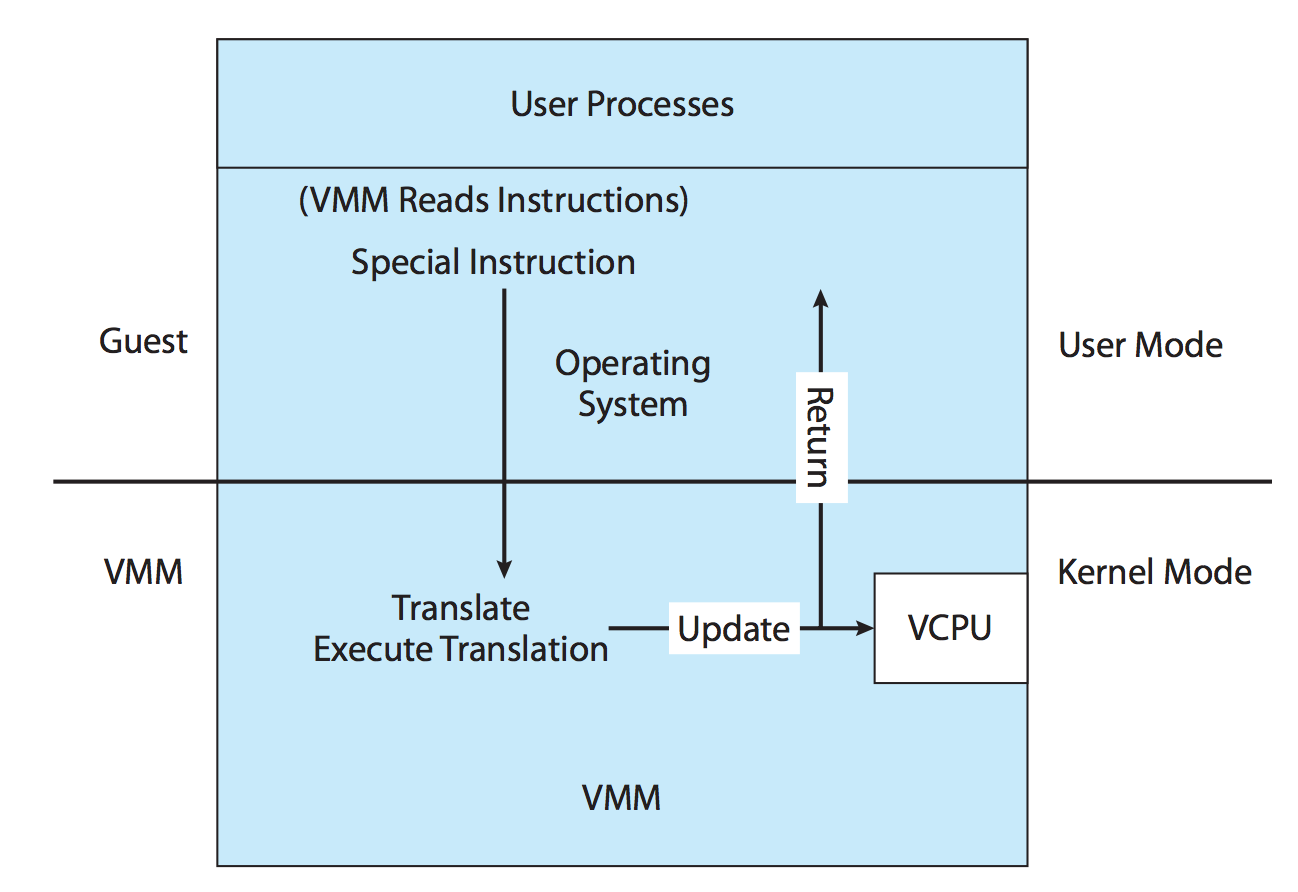
\includegraphics[width=0.75\textwidth]{images/binary-translation.png}
\end{center}


\end{frame}

\begin{frame}
\frametitle{Binary Translation Performance}

We have a performance decrease as a result of having to examine and replace some of the instructions. 

Most instructions can run natively; only a small number need to be emulated. 

The empirical test of ``what is being used in industry'' seems to indicate that the performance of binary translation is adequate. 

There is now widespread adoption of virtual machines running x86 hardware.


\end{frame}

\begin{frame}
\frametitle{One More Hardware Rescue}

Additional hardware support makes virtualization work a lot better.

In 2005, Intel added virtualization support to x86; AMD added it in 2006. 

This changes dual-mode (kernel/user) processors into multi-mode operation. 

The VMM can enable host mode, define a guest's characteristics, and then switch to guest mode, passing control to the guest. 

If the guest tries to access a virtualized resource, the VMM takes over.


\end{frame}

\begin{frame}
\frametitle{The Impact of Virtualization}

The short version of what happens under virtualization is:\\
\quad Things get complicated. 

There are more demands on and difficulties in resources. 

We will consider the impact on scheduling, memory management, I/O, disk.

\end{frame}

\begin{frame}
\frametitle{Virtualized Scheduling}

Even if there is only one CPU in the physical machine, virtualization presents one or more virtual CPUs to the guests. 

The challenge is to schedule the virtual CPUs' operations on physical CPU(s). 

A thread may be a VMM thread or a guest thread.

\end{frame}



\begin{frame}
\frametitle{CPU Assignment}


A guest system is configured with some number of CPUs.

As long as there are enough CPUs in the system to meet the allocation commitments (virtual CPU count is less than $n$), we have no problem. 


Map each virtual CPU to a physical CPU and we are all set. 

\end{frame}

\begin{frame}
\frametitle{CPU Assignment}

If the resources are fully committed (e.g., there are $n$ virtual CPUs allocated), it gets a bit more interesting. 

The VMM does not (usually) need too much time on its own, so it can basically ``steal'' cycles here and there. 

VMM operations run on CPUs that are not busy at the moment, or taking evenly from all the CPUs so as to be ``fair''. 


\end{frame}

\begin{frame}
\frametitle{CPU Overcommitment}

If the situation is overcommitted (there are more virtual CPUs than physical ones), the problem is more interesting. 

The VMM will have to figure out a way to map the virtual CPUs to the physical ones according to some scheduling strategy. 

Like scheduling processes/threads, we can use a scheduling algorithm.

\end{frame}

\begin{frame}
\frametitle{CPU Overcommitment}

When overcommitment is the situation, the expectation of the guest operating system of certain time deadlines becomes inaccurate. 

If the scheduler in the guest operating system defines a timeslice as, for example, 50~ms, in reality the actual length of a time slice will vary. 

It could, in fact, be significantly longer than the 50~ms intended. 

This is has a tendency to get the system clock out of whack, but may be fatal for any real-time operating system or any task with serious wall-clock deadlines.

\end{frame}

\begin{frame}
\frametitle{Virtualized Memory Management}

Virtualization makes the memory problem a lot worse.

The processes that run take up plenty of memory all on their own. 

Now there are multiple operating systems and their structures taking up memory space, too. 

The problem is only exacerbated if memory is overcommitted.

\end{frame}

\begin{frame}
\frametitle{Nested Page Tables}

The guest operating system, unaware it is in a virtual machine, thinks it controls memory and page table management. 

In reality, the virtual machine manager has a nested page table that re-translates the guest's page  table to the real (physical) page table. 

The VMM can provide double-paging, where it has its own page replacement strategy and tries to help out the guest.

The problem is that the VMM knows less about the guest's memory patterns than the guest itself, so this strategy is inefficient.


\end{frame}

\begin{frame}
\frametitle{Device Driver}

The next idea is then to install, where possible, a device driver into the guest that allows the VMM to exercise some measure of control over the guest. 

When needed, this ``balloon'' memory manager is told to request a whole bunch of (empty) memory and asks the guest to pin its pages in physical memory. 

This makes the guest think that memory is in short supply;\\
\quad The guest will start to free up memory. 

The VMM knows that the balloon pages are not real and can allocate them to some other guest. 

If the memory pressure in the whole system goes down, the balloon pages can be deallocated, allowing the guest to feel as if it has more free memory.

\end{frame}



\begin{frame}
\frametitle{Duplicate Detection}

Idea: look to see if the same page is loaded more than once. 

This is obviously more likely if the guests are identical (i.e., the same OS). 

This will result in significant savings, as the operating system may take up a significant portion of memory on its own. 

A hash value for memory may be taken; if two hashes match then a byte-by-byte comparison will reveal whether they are actually identical. 

If there is a modification to a shared page, we need to copy the page before the modification is made.


\end{frame}

\begin{frame}
\frametitle{Virtualized I/O Devices}

Unlike CPUs and RAM, the guest OSes are likely to tolerate the fact that the I/O devices may change periodically and during operation.

Example: when a user plugs in a USB key or moves into range of a WiFi network. 

When running in a virtual machine, a guest may see several virtual devices as if they were real.


\end{frame}

\begin{frame}
\frametitle{Virtualized I/O Devices}

The VMM can decide how to allocate I/O devices to guests. 

One way is to just dedicate the I/O device to a guest such as a USB key being allocated to one guest in particular. 

In other cases, the VMM provides drivers that are just translating commands into the actual device commands. 

\end{frame}

\begin{frame}
\frametitle{Virtualized Disk}

The typical approach is to create a \alert{disk image}, that contains all the contents of the root disk of the guest. 

This is one big file (though it can be split up into manageable-sized chunks) and as far as the guest is concerned it has the run of that whole disk.

The guest is totally unaware that the disk is just a file inside another system. 

This makes it easy to move a virtual machine from one system to another.
\end{frame}

\begin{frame}
\frametitle{Containerize Me, Captain}

\begin{center}
	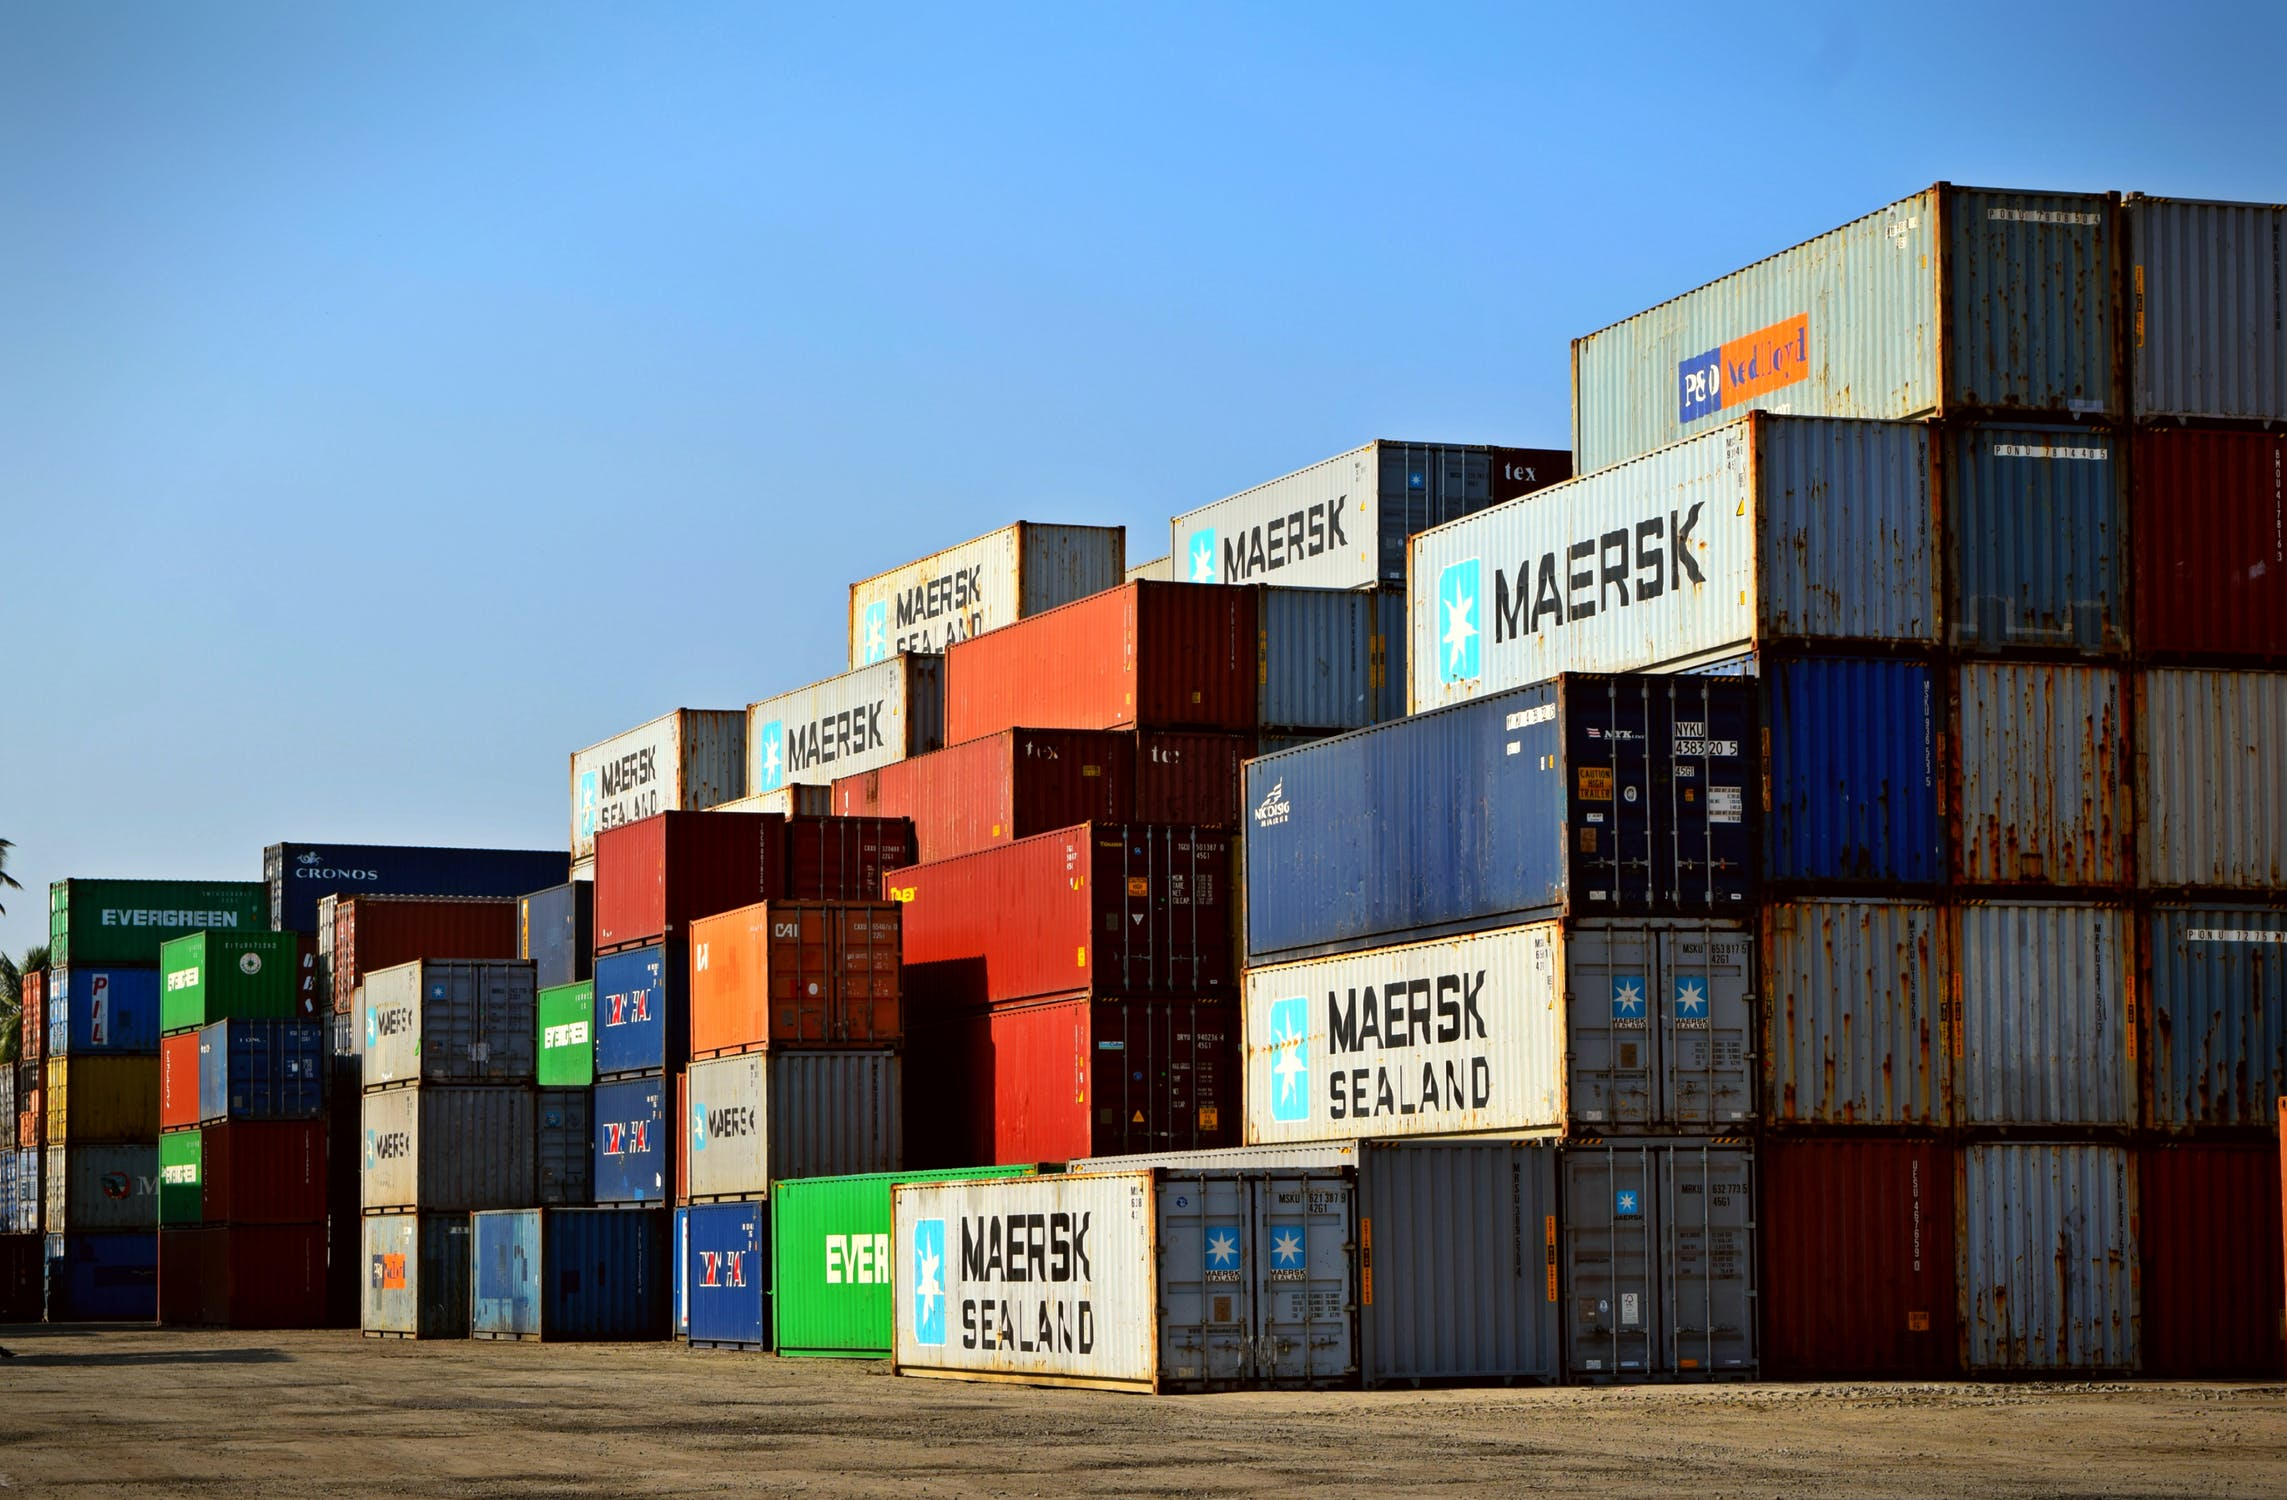
\includegraphics[width=0.7\textwidth]{images/container.jpeg}
\end{center}

\end{frame}


\begin{frame}
\frametitle{How Did We Get Here?}

\begin{itemize}
	\item Manual install
	\item Package Manager (RPM/JAR/DLL Hell)
	\item Virtual Machines
	\item Containerization
\end{itemize}


\end{frame}


\begin{frame}
\frametitle{Containers}

See this diagram from NetApp:

\begin{center}
	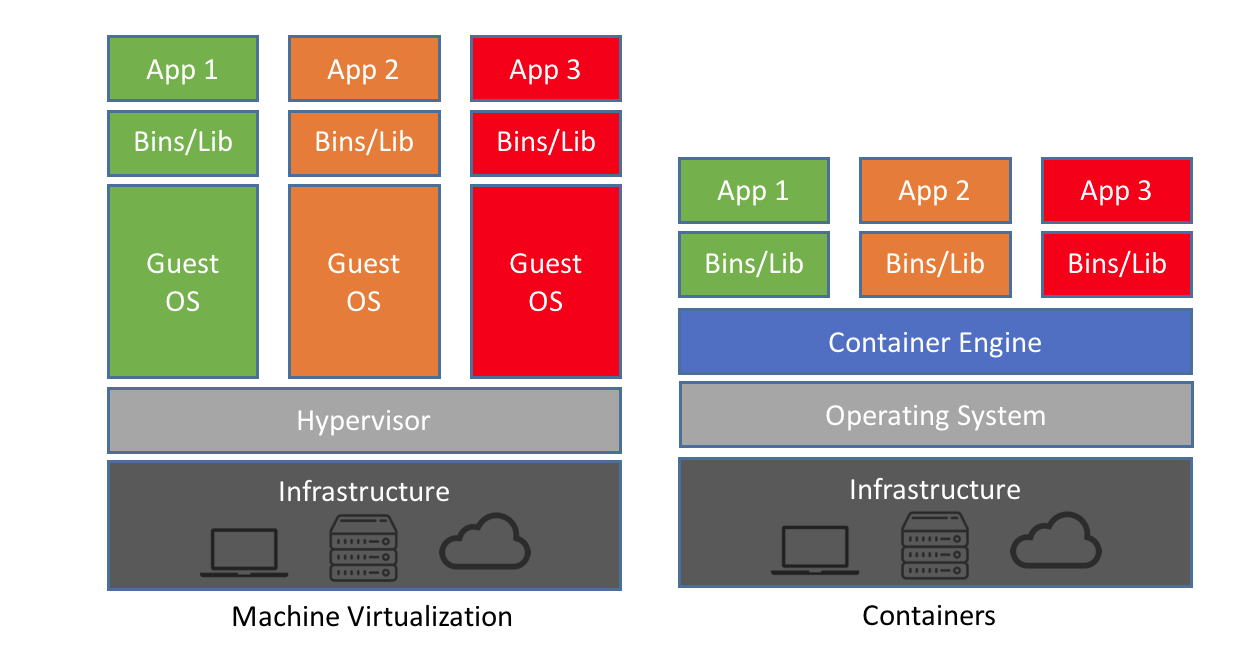
\includegraphics[width=0.7\textwidth]{images/cvm.png}
\end{center}


\end{frame}



\end{document}

